%%%%%%%%%%%%%%%%%%%%%%%%%%%%%%%%%%%%%%%%%%%%%%%%%%%%%%%%%%%%%%%%%
% MUW Presentation
% LaTeX Template
% Version 1.0 (27/12/2016)
%
% License:
% CC BY-NC-SA 4.0 (http://creativecommons.org/licenses/by-nc-sa/3.0/)
%
% Created by:
% Nicolas Ballarini, CeMSIIS, Medical University of Vienna
% nicoballarini@gmail.com
% http://statistics.msi.meduniwien.ac.at/
%
% Customized for UAH by:
% David F. Barrero, Departamento de Automática, UAH
%%%%%%%%%%%%%%%%%%%%%%%%%%%%%%%%%%%%%%%%%%%%%%%%%%%%%%%%%%%%%%%%%

\documentclass[10pt,compress]{beamer} % Change 10pt to make fonts of a different size
\mode<presentation>

\usepackage[spanish]{babel}
\usepackage{fontspec}
\usepackage{tikz}
\usepackage{etoolbox}
\usepackage{xcolor}
\usepackage{xstring}
\usepackage{listings}

% Custom packages
\usepackage{svg}
\usepackage{standalone}
\usepackage{multicol}
\usepackage{multirow} % Confusion matrix
\usepackage{tikz}
\usepackage{pgfplots}
\def\layersep{2.5cm}
\usetikzlibrary{matrix,chains,positioning,decorations.pathreplacing,arrows,shapes}

\definecolor{dkgreen}{rgb}{0,0.6,0}
\definecolor{gray}{rgb}{0.5,0.5,0.5}
\definecolor{mauve}{rgb}{0.58,0,0.82}
 

\usetheme{UAH}
\usecolortheme{UAH}
\setbeamertemplate{navigation symbols}{} 
\setbeamertemplate{caption}[numbered]

%%%%%%%%%%%%%%%%%%%%%%%%%%%%%%%%%%%%%%%%%%%%%%%%%%%%%%%%%%%%%%%%%
%% Presentation Info
\title[Unsupervised learning]{Unsupervised learning}
\author{\asignatura\\\carrera}
\institute{}
\date{Departamento de Automática}
%%%%%%%%%%%%%%%%%%%%%%%%%%%%%%%%%%%%%%%%%%%%%%%%%%%%%%%%%%%%%%%%%


%%%%%%%%%%%%%%%%%%%%%%%%%%%%%%%%%%%%%%%%%%%%%%%%%%%%%%%%%%%%%%%%%
%% Descomentar para habilitar barra de navegación superior
\setNavigation
%%%%%%%%%%%%%%%%%%%%%%%%%%%%%%%%%%%%%%%%%%%%%%%%%%%%%%%%%%%%%%%%%

%%%%%%%%%%%%%%%%%%%%%%%%%%%%%%%%%%%%%%%%%%%%%%%%%%%%%%%%%%%%%%%%%
%% Configuración de logotipos en portada
%% Opacidad de los logotipos
\newcommand{\opacidad}{1}
%% Descomentar para habilitar logotipo en pié de página de portada
\renewcommand{\logoUno}{Images/isg.png}
%% Descomentar para habilitar logotipo en pié de página de portada
%\renewcommand{\logoDos}{Images/CCLogo.png}
%% Descomentar para habilitar logotipo en pié de página de portada
%\renewcommand{\logoTres}{Images/ALogo.png}
%% Descomentar para habilitar logotipo en pié de página de portada
%\renewcommand{\logoCuatro}{Images/ELogo.png}
%%%%%%%%%%%%%%%%%%%%%%%%%%%%%%%%%%%%%%%%%%%%%%%%%%%%%%%%%%%%%%%%%

%%%%%%%%%%%%%%%%%%%%%%%%%%%%%%%%%%%%%%%%%%%%%%%%%%%%%%%%%%%%%%%%%
%% FOOTLINE
%% Comment/Uncomment the following blocks to modify the footline
%% content in the body slides. 


%% Option A: Title and institute
\footlineA
%% Option B: Author and institute
%\footlineB
%% Option C: Title, Author and institute
%\footlineC
%%%%%%%%%%%%%%%%%%%%%%%%%%%%%%%%%%%%%%%%%%%%%%%%%%%%%%%%%%%%%%%%%


\begin{document}

%%%%%%%%%%%%%%%%%%%%%%%%%%%%%%%%%%%%%%%%%%%%%%%%%%%%%%%%%%%%%%%%%
% Use this block for a blue title slide with modified footline
{\titlepageBlue
    \begin{frame}
        \titlepage
    \end{frame}
}

\institute{\asignatura}

\begin{frame}[plain]{}
   \begin{block}{Objectives}
      \begin{enumerate}
         \item TODO
      \end{enumerate} 
   \end{block}

   \begin{block}{Bibliography}
	\begin{itemize}
        \item TODO Bishop, Christopher M. \textit{Pattern Recognition and Machine Learning}. 2nd edition. Springer-Verlag. 2011
        \item TODO M\"uller, Andreas C., Guido, Sarah. \textit{Introduction to Machine Learning with Python}. O'Reilly. 2016
	\end{itemize}
   \end{block}
\end{frame}

{
\disableNavigation{white}
\begin{frame}[shrink]{Table of Contents}

 	\frametitle{Table of Contents}
  	\begin{multicols}{2}
  		\tableofcontents
    \end{multicols}

 %\frametitle{Table of Contents}
 %\tableofcontents
  % You might wish to add the option [pausesections]
\end{frame}
}

%%%%%%%%%%%%%%%%%%%%%%%%%%%%%%%%%%%%%%%%%%%%%%%%%%%%%%%%%%%%%%%%%
\section{Clustering}
{
\sectionheaderWhite %Enclose the frame with {} and add this command for white background in section header
\begin{frame}{Clustering}{K-means, agglomerative clustering, DBSCAN and GMM}
\end{frame}
}

\subsection{Aplications}
\begin{frame}{Clustering}{Applications}
	Set of unsupervised techniques that identify groups of data (named \alert{clusters})
    \begin{itemize}
        \item No universal definition of cluster: Centroid, medoid, dense regions, etc
    \end{itemize}

    Applications
	\begin{itemize}
		\item Customer segmentation
           \item Data analysis
           \item Dimensionality reduction
           \item Anomaly detection
           \item Semi-supervised learning
           \item Search engines
           \item Image segmentation
	\end{itemize}

    Main algorithms
	\begin{itemize}
		\item K-means, DBScan, GMM, hierarchical clustering, EM, ...
	\end{itemize}
\end{frame}

\section{K-means}
\subsection{Overview}
\begin{frame}{K-means}{Overview}
    \begin{columns}
 	   \column{.5\textwidth}
       \centering Original data\\
		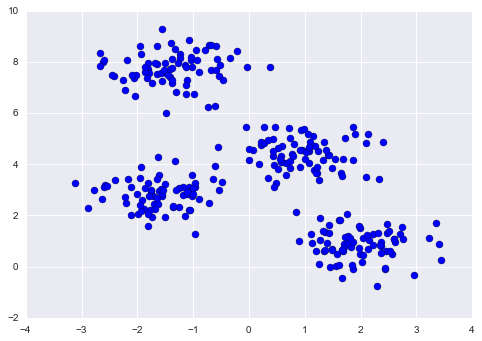
\includegraphics[width=\textwidth]{figs/kmeans-1.png}
 	   \column{.5\textwidth}
       \centering Clustered data\\
		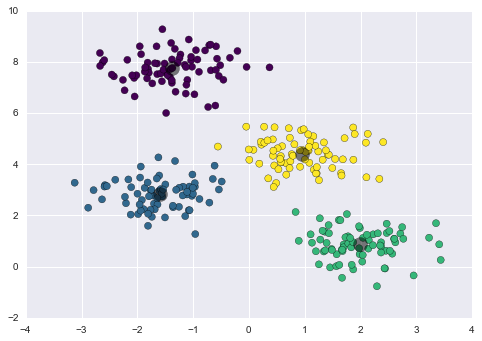
\includegraphics[width=\textwidth]{figs/kmeans-2.png}
    \end{columns}

    \centering \tiny{\href{https://jakevdp.github.io/PythonDataScienceHandbook/05.11-k-means.html}{(Source)}}

    \normalsize
    \begin{flushleft}
    In k-means, clusters are identified by a \alert{centroid}
    \end{flushleft}
\end{frame}

\subsection{K-means algorithm}
\begin{frame}{K-means}{K-means algorithm (I)}
    \begin{columns}
 	   \column{.5\textwidth}
       \begin{block}{K-means algorithm}
       \begin{enumerate}
        \item Set $k$ random centroids
        \item Assign each data point to its closest centroid
        \item Recompute centroids
        \item Go to 2 until no point reassignment
       \end{enumerate}
       \end{block}

       k is an hyperparameter
       \begin{itemize}
        \item Number of clusters
       \end{itemize}

 	   \column{.5\textwidth}
		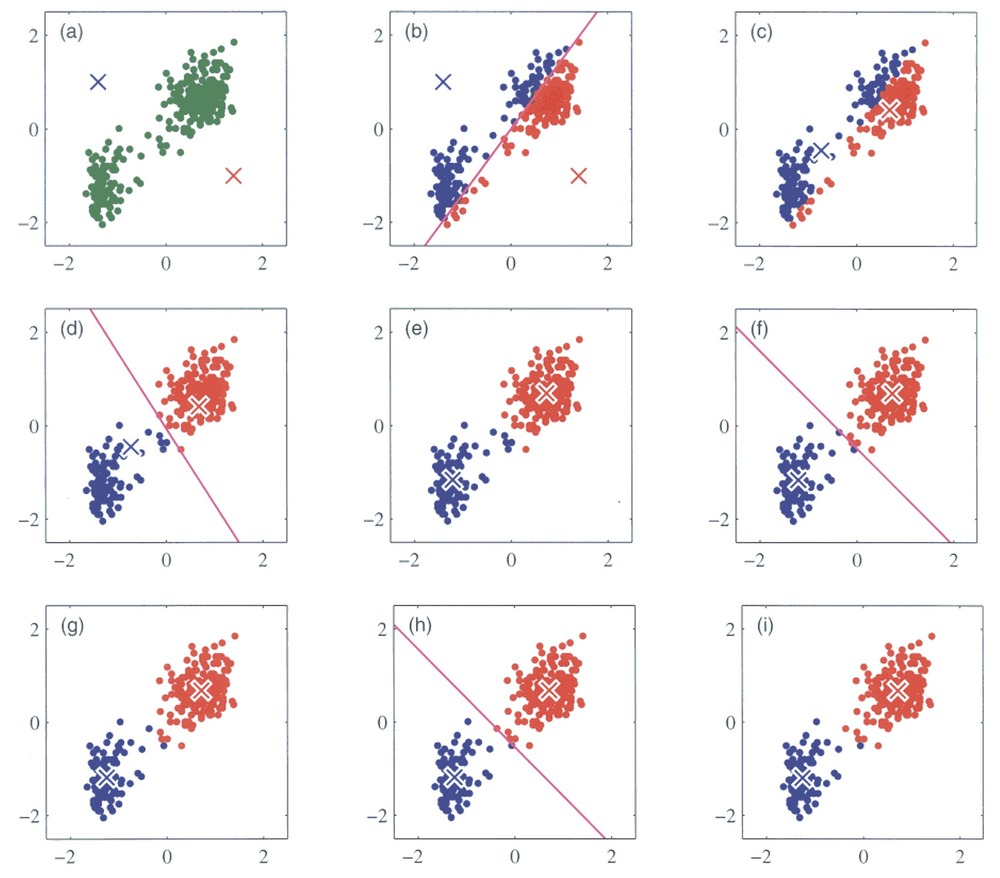
\includegraphics[width=\textwidth]{figs/kmeans.jpeg}\\

    \centering \tiny{\href{https://dendroid.sk/2011/05/09/k-means-clustering/}{(Source)}}
    \end{columns}

\end{frame}

\begin{frame}{K-means}{K-means algorithm (II)}
    New data points are assigned to its closest centroid
    \begin{columns}
 	   \column{.5\textwidth}
		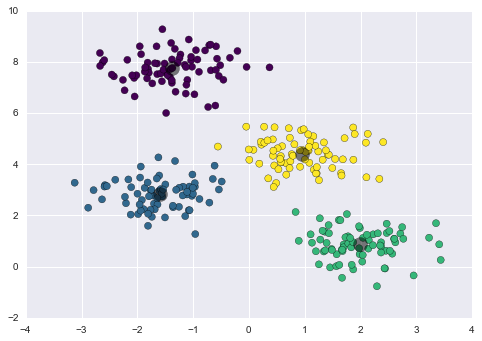
\includegraphics[width=\textwidth]{figs/kmeans-2.png}

 	   \column{.5\textwidth}
		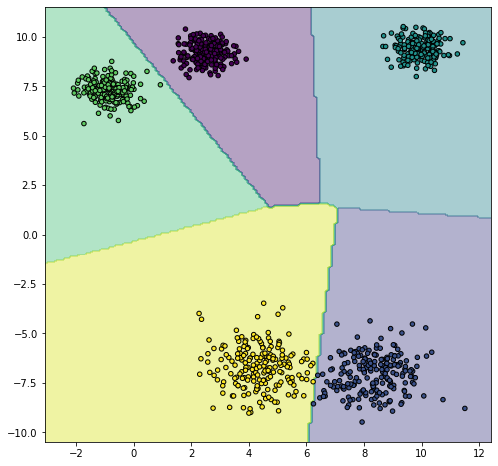
\includegraphics[width=\textwidth]{figs/voronoi.png}
    \end{columns}
\end{frame}

\subsection{K-means limitations}
\begin{frame}{K-means}{K-means limitations}
    \begin{columns}
 	   \column{.5\textwidth}
    K-means can fail in several conditions
       \begin{itemize}
        \item Incorrect number of clusters
        \item Different clusters variance
        \item Non-spheric clusters $\Rightarrow$ normalization
       \end{itemize}
 	   \column{.5\textwidth}
	\centering 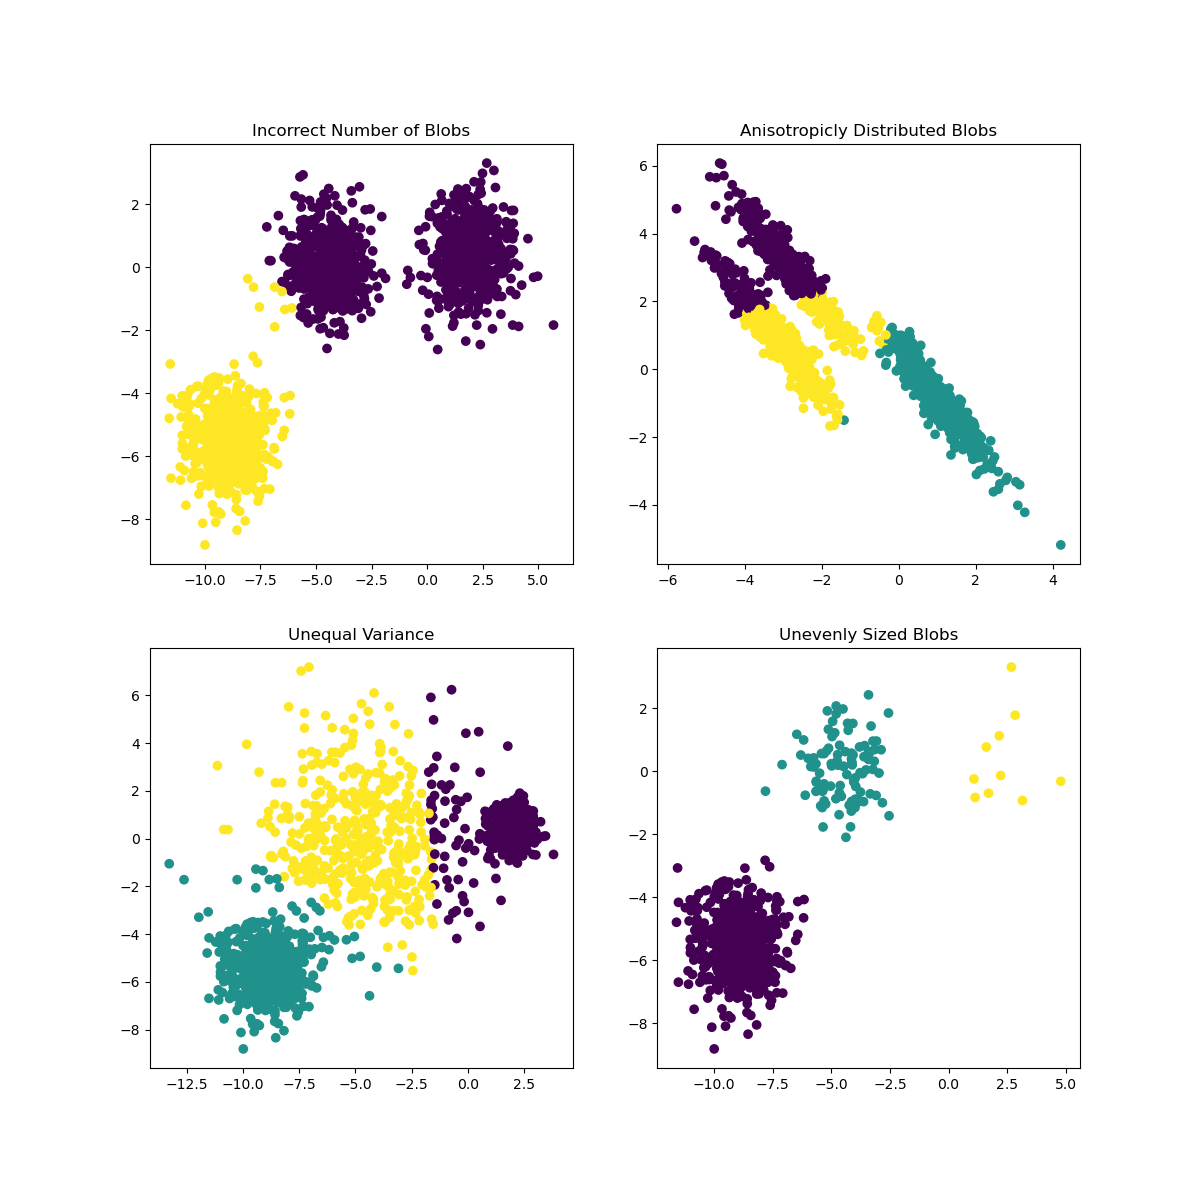
\includegraphics[width=\textwidth]{figs/kmeans-fails.png}\\
    \tiny{\href{https://scikit-learn.org/stable/auto_examples/cluster/plot_kmeans_assumptions.html}{(Source)}}
    \end{columns}
\end{frame}

\subsection{Elbow's method}
\begin{frame}{K-means}{Elbow's method}
    Election of $k$
    \begin{itemize}
        \item Not a problem when domain information is available
        \item ... that is rarely the case
    \end{itemize}

    \begin{columns}
 	   \column{.50\textwidth}
        \begin{block}{Elbow's method}
           \begin{enumerate}
            \item Select $K=1, ..., n$
            \item Visualize performance for each k
            \item Choose K where metric stabilizes
           \end{enumerate} 
        \end{block}
 	   \column{.50\textwidth}
			\begin{figure}
		        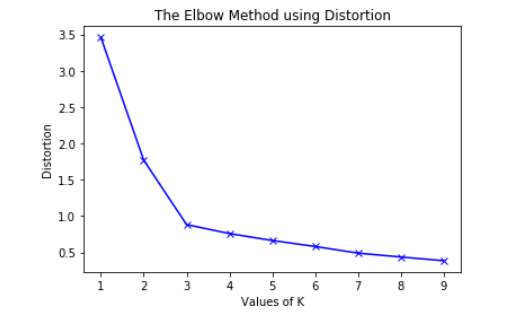
\includegraphics[width=\textwidth]{figs/elbow.png}
			\end{figure}
    \end{columns}

    Performance measures
    \begin{itemize}       
        \item Inertia: mean squared error between each instance and its closest centroid
        \item Silhouette: $(b-a) / max (a, b)$, where $a$ mean intra-cluster distance, and $b$ is the mean nearest-cluster distance
    \end{itemize}       
\end{frame}

\subsection{Application: Image segmentation}
\begin{frame}[plain]{K-means}{Application: Image segmentation}
	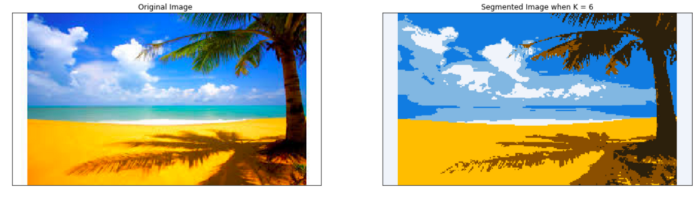
\includegraphics[width=0.8\textwidth]{figs/segmentation1.png}\\
        \centering \tiny{\href{https://www.kdnuggets.com/2019/08/introduction-image-segmentation-k-means-clustering.html}{(Source)}}

    \medskip

	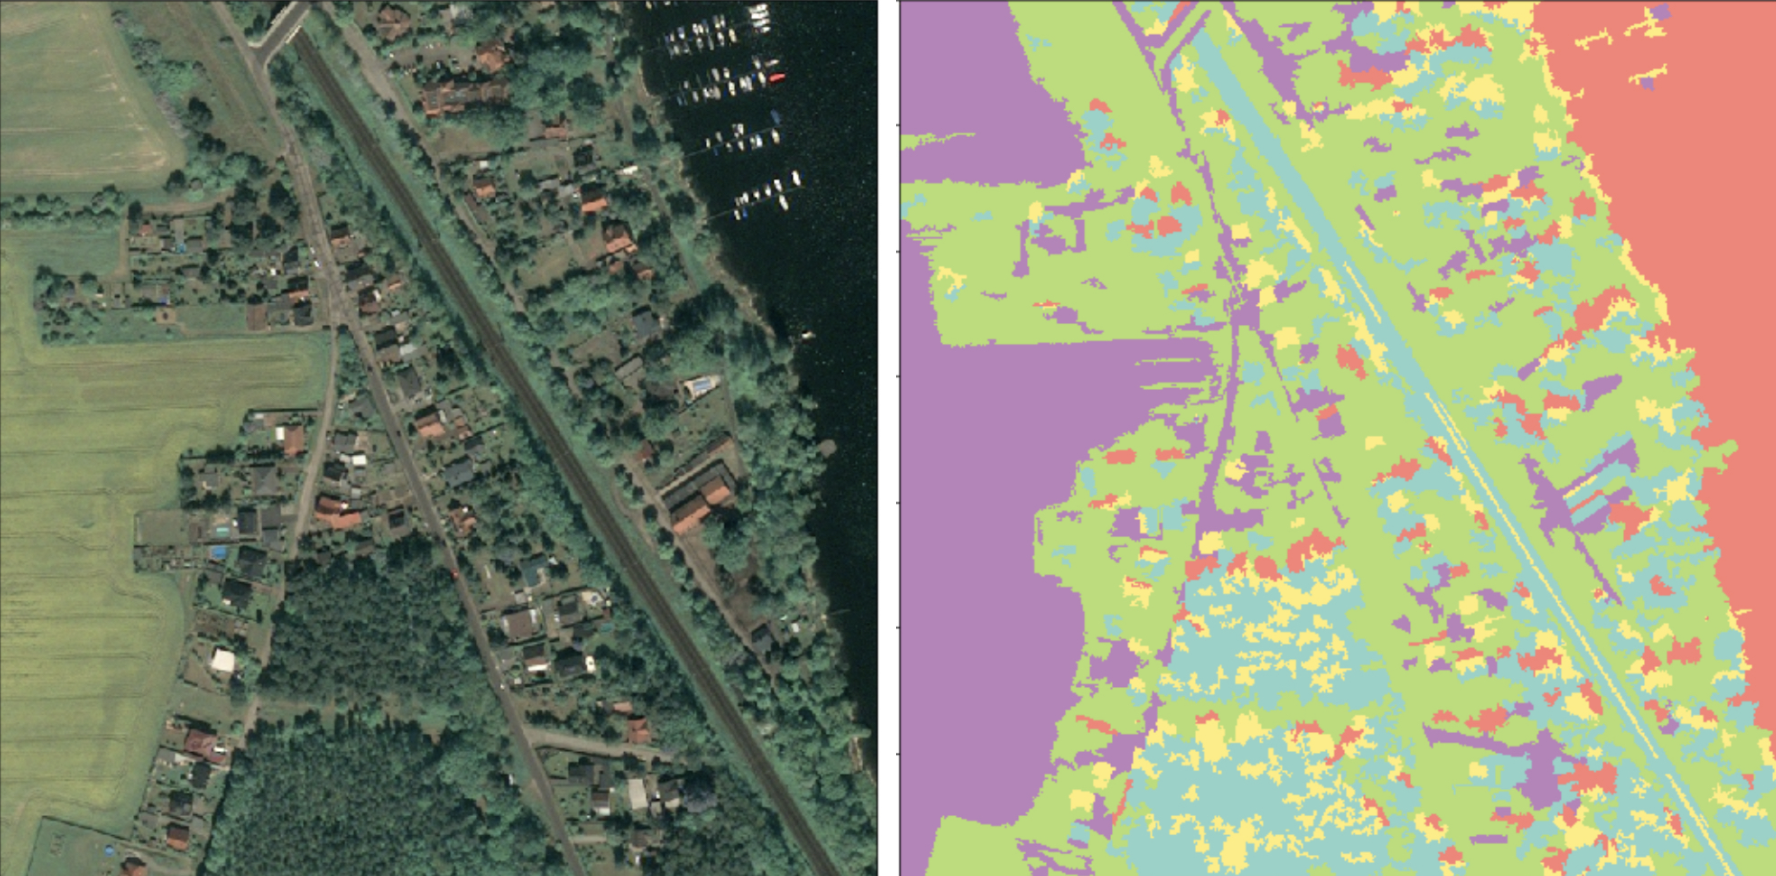
\includegraphics[width=0.8\textwidth]{figs/segmentation2.png}\\
        \centering \tiny{\href{https://up42.com/blog/tech/satellite-image-processing-made-simple}{(Source)}}
\end{frame}

\subsection{Application: for semi-supervised learning}
\begin{frame}[plain]{K-means}{Application: Clustering for semi-supervised learning}
    Semi-supervised learning: Only a subset of the dataset is labeled
    \begin{itemize}
       \item Supervised and unsupervised learning
       \item Quite common in real-world applications (labels use to be expensive)
    \end{itemize} 

	\begin{center}
	\begin{tabular}{cccccc}\hline
	 	$f_1$     & $f_2$     & $\cdots$ & $f_n$     & $y$\\\hline
	 	$a_{1,1}$ & $a_{2,1}$ & $\cdots$ & $a_{n,1}$ & $y_1$ \\
	 	$a_{1,2}$ & $a_{2,2}$ & $\cdots$ & $a_{n,2}$ &  \\
	 	$a_{1,3}$ & $a_{2,3}$ & $\cdots$ & $a_{n,3}$ &  \\
	 	$a_{1,4}$ & $a_{2,4}$ & $\cdots$ & $a_{n,4}$ & $y_4$ \\
	 	$a_{1,5}$ & $a_{2,5}$ & $\cdots$ & $a_{n,5}$ &  \\
	 	\hline
	\end{tabular}
	\end{center}

    \begin{block}{Label propagation}
    \begin{enumerate}
       \item Obtain $k$ clusters
       \item Get a representative instance of each cluster (\alert{medoid}) measuring the distance to the centroid
       \item Label the members of each cluster with its medoid's label
    \end{enumerate} 
    \end{block}
\end{frame}

\IfStrEq{\modo}{muii}{
    \subsection{K-means: Scikit-Learn}
    \begin{frame}{Clustering}{K-means: Scikit-learn}
        TODO: SCikit-Learn
    \end{frame}
}{}

\subsection{K-means summary}
\begin{frame}[fragile]{K-means}{K-means: Summary}
	\begin{center}
	\begin{tabular}{cll}\hline
	 	\texttt{Hyperparameters}  & \texttt{Advantages}  & \texttt{Disadvantages} \\\hline
	 	                 & Fast                 & Simple shapes \\
	    $k$	             & Few hyperparameters  & Determine $k$ \\
	 	                 & Scalable             & Random initialization \\
	 	\hline
	\end{tabular}
	\end{center}
\end{frame}


\section{Other clustering algorithms}

\subsection{GMM}

\begin{frame}{Other clustering algorithms}{Gaussian Mixure Model (GMM) (I)}
	GMM is a generative clustering algorithm
	\begin{itemize}
		\item Assumes data coming from a set of multidimensional gaussian distributions
	\end{itemize}

    GMM fits a set $\{(\phi_i, \mu_i, \sigma_i)\}_{i=1,\dots, k}$
	\begin{itemize}
			\item $\phi$ is a weight
			\item $\mu$ is a multidimensional mean
			\item $\sigma$ is a covariance matrix
            \item $k$ is the number of clusters (hyperparameter)
	\end{itemize}

	\bigskip
	\centering 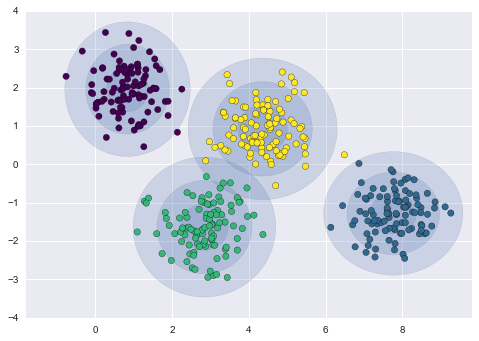
\includegraphics[width=0.31\linewidth]{figs/gmm2.png}
	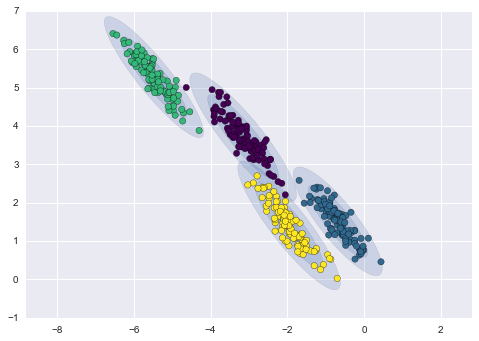
\includegraphics[width=0.31\linewidth]{figs/gmm3.png}\\
	%\centering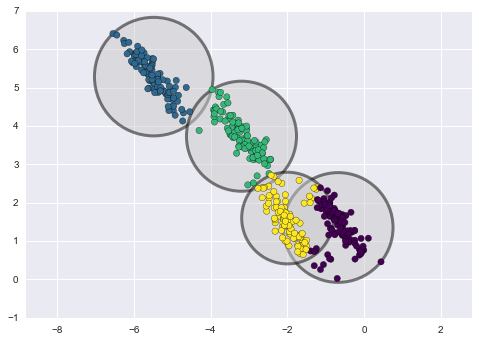
\includegraphics[width=0.31\linewidth]{figs/gmm1.png}\\
	\scriptsize\href{https://jakevdp.github.io/PythonDataScienceHandbook/05.12-gaussian-mixtures.html}{(Source)}
\end{frame}

\begin{frame}{Other clustering algorithms}{Gaussian Mixure Model (GMM) (II)}
    Gaussian parameters are fit with the Expectation-Maximization (E-M) algorithm
       \begin{itemize}
            \item E-M is a generalization of K-means
       \end{itemize}

    \begin{block}{Expectation-Maximization algorithm}
    \begin{enumerate}
       \item Init parameters randomly
       \item Expectation step: Assign each instance to a cluster
            \begin{itemize}
            \item Assignment is probabilistic
            \end{itemize}
       \item Maximization step: Update cluster parameters
            \begin{itemize}
            \item Each cluster is updated using \textit{all} the data
            \item Instances contribution to a cluster parameters is weighted by the probability that it belongs to it
            \end{itemize}
       \item Go to 2
    \end{enumerate} 
    \end{block}

    GMM can be seen as a fuzzy clustering algorithm
\end{frame}

\begin{frame}{Other clustering algorithms}{Gaussian Mixure Model (GMM) (III)}
    Gaussian parameters are fit with the Expectation-Maximization (E-M) algorithm
       \begin{itemize}
            \item E-M is a generalization of K-means
       \end{itemize}

    \begin{block}{Expectation-Maximization algorithm}
    \begin{enumerate}
       \item Init parameters randomly
       \item Expectation step: Assign each instance to a cluster
            \begin{itemize}
            \item Assignment is probabilistic
            \end{itemize}
       \item Maximization step: Update cluster parameters
            \begin{itemize}
            \item Each cluster is updated using \textit{all} the data
            \item Instances contribution to a cluster parameters is weighted by the probability that it belongs to it
            \end{itemize}
       \item Go to 2
    \end{enumerate} 
    \end{block}

    GMM can be seen as a fuzzy clustering algorithm
\end{frame}


\begin{frame}{Other clustering algorithms}{Gaussian Mixure Model (GMM) (IV)}
    GMM provides a probability of an instance to belong to a cluster
    \begin{itemize}
         \item This can be used to detect anomalies
         \item Just assign a probability threshold
    \end{itemize} 
    
    \bigskip

    \centering
	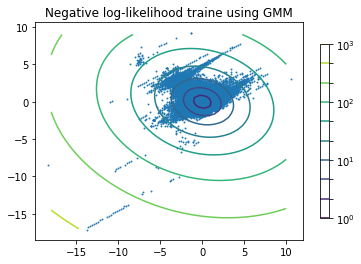
\includegraphics[width=0.4\textwidth]{figs/gmm-anomaly.png}
	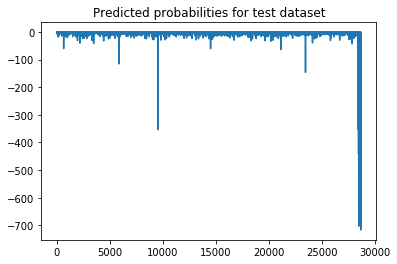
\includegraphics[width=0.4\textwidth]{figs/gmm-anomaly2.png}\\
	\scriptsize\href{https://www.kaggle.com/code/albertmistu/detect-anomalies-using-gmm}{(Source)}
\end{frame}

\IfStrEq{\modo}{muii}{
    \subsection{DBSCAN: Scikit-Learn}
    \begin{frame}{Other clustering algorithms}{DBSCAN: Scikit-learn}
        TODO: Scikit-Learn
    \end{frame}
}{}

\begin{frame}{Other clustering algorithms}{GMM: Summary}
	\begin{center}
	\begin{tabular}{cp{3cm}p{3cm}}\hline
	 	\texttt{Hyperparameters}  & \texttt{Advantages}      & \texttt{Disadvantages} \\\hline
	 	Number of clusters        & Probabilistic clustering & Number of clusters \\
	    Covariance matrix type	  & Generative model         & Gaussian data \\
	    	                      & Anomaly detection        & Sensitive to outliers \\
	 	\hline
	\end{tabular}
	\end{center}
\end{frame}


\subsection{DBSCAN}

\begin{frame}{Other clustering algorithms}{DBSCAN (I)}
	DBSCAN: Density-Based Spatial Clustering of Applications with Noise
	\begin{itemize}
		\item Identifies high density regions (dense regions) in feature space
        \item Asumtion: Clusters form dense regions separated by empty areas
	\end{itemize}
    Hyperparameters
    \begin{itemize}
        \item $\epsilon$: Radius of a neighborhood
        \item $min\_samples$: Minumun cluster size
    \end{itemize}

    Type of points
    \begin{itemize}
        \item Core instance
        \item Outliers
    \end{itemize}

    \vspace{-3cm}
	\begin{flushright} 
        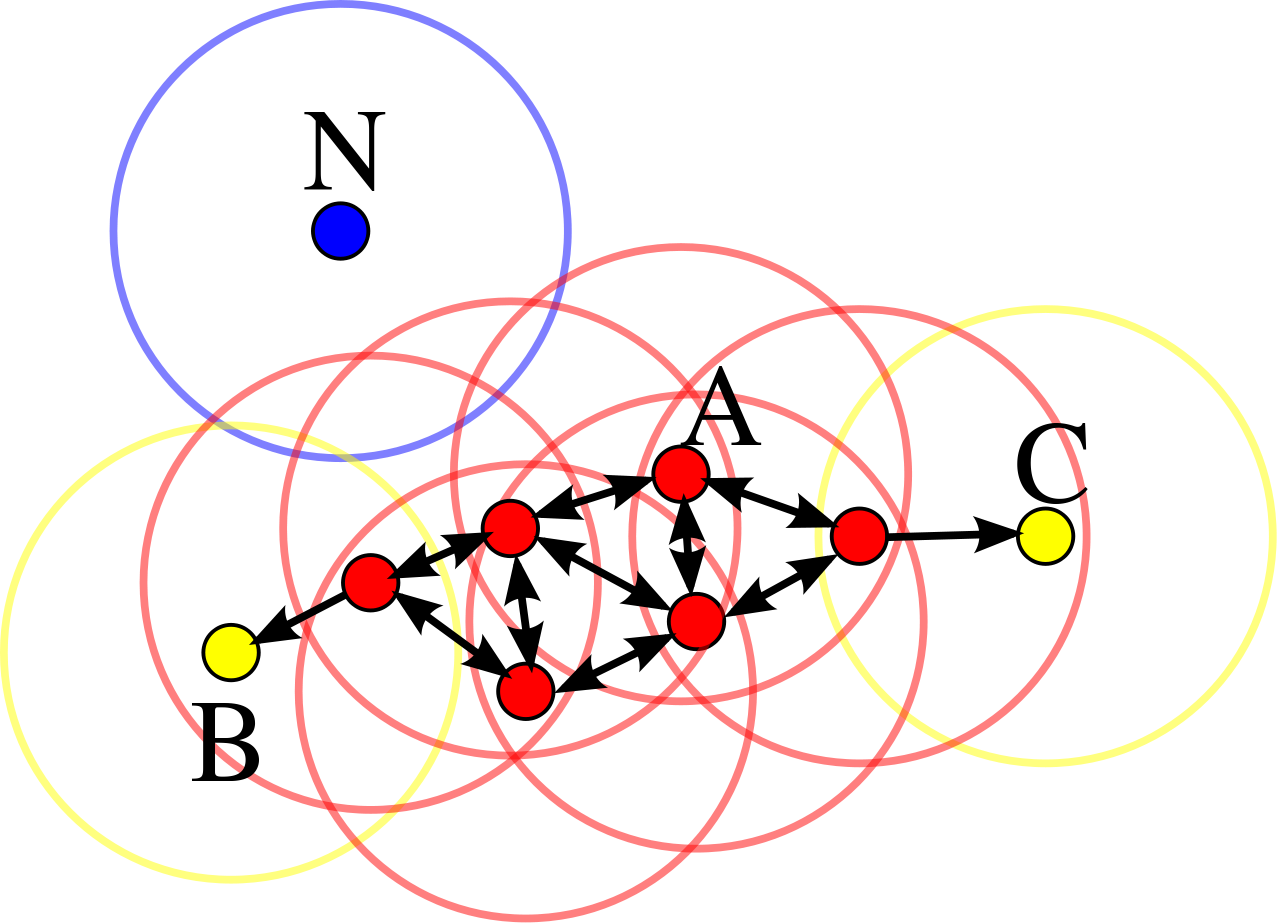
\includegraphics[width=0.5\linewidth]{figs/dbscan.png}
	    \scriptsize\href{https://en.wikipedia.org/wiki/DBSCAN}{(Source)}\hspace{20cm}
    \end{flushright}
\end{frame}

%\begin{frame}{Other clustering algorithms}{DBSCAN (II)}
%    \begin{columns}
% 	   \column{.5\textwidth}
%       \begin{block}{DBSCAN algorithm}
%            \begin{enumerate}
%                \item For each instance, take the neighbors located within a distance of $\epsilon$
%                \item If it has $>min_samples$ neighbors, consider it as core instance
%            \end{enumerate}
%       \end{block}
%    \end{columns}
%\end{frame}

\begin{frame}{Other clustering algorithms}{DBSCAN (II)}
    \begin{columns}
 	   \column{.5\textwidth}
        \centering $\epsilon$=0.05, $min\_samples=5$\\
	    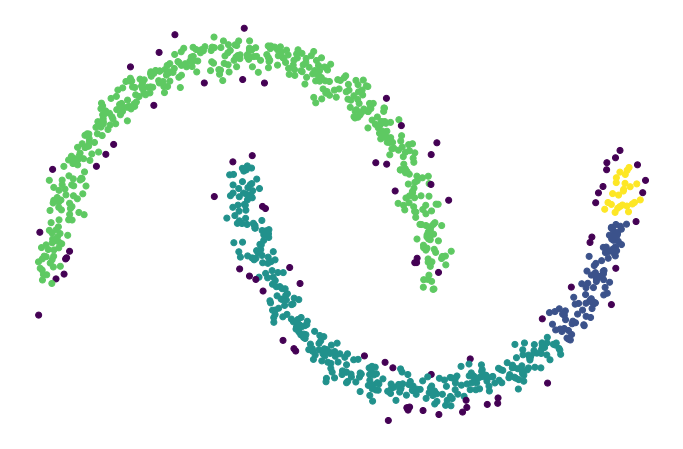
\includegraphics[width=\textwidth]{figs/dbscan1.png}\\
        
 	   \column{.5\textwidth}
       \centering $\epsilon$=0.2, $min\_samples=5$\\
	   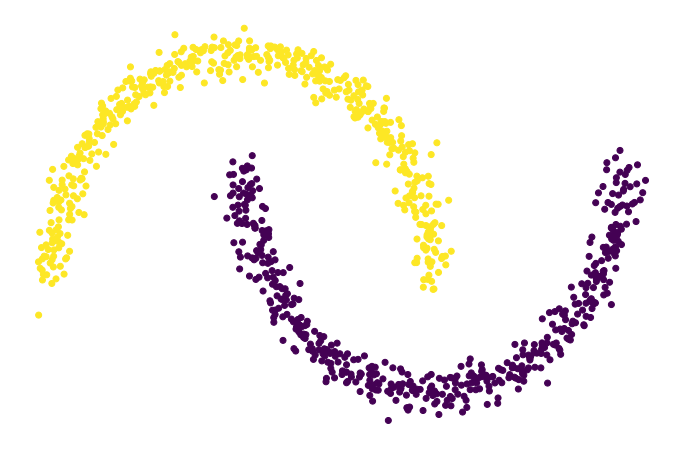
\includegraphics[width=\textwidth]{figs/dbscan2.png}\\
    \end{columns}
    \centering \tiny{\href{https://github.com/Akramz/Hands-on-Machine-Learning-with-Scikit-Learn-Keras-and-TensorFlow/blob/master/09.Unsupervised_learning.ipynb}{(Source)}}
\end{frame}

\IfStrEq{\modo}{muii}{
    \subsection{DBSCAN: Scikit-Learn}
    \begin{frame}{Other clustering algorithms}{DBSCAN: Scikit-learn}
        TODO: Scikit-Learn
    \end{frame}
}{}


\subsection{Summary}
\begin{frame}{Other clustering algorithms}{DBSCAN: Summary}
	\begin{center}
	\begin{tabular}{cp{3cm}p{3cm}}\hline
	 	\texttt{Hyperparameters}  & \texttt{Advantages}    & \texttt{Disadvantages} \\\hline
	 	$\epsilon$                & No explicit number of clusters  & Slower than K-means \\
	    $min\_samples$	          & Scales relatively well & Clusters with different densities \\
	                 	          & Almost deterministic   &  \\
	                 	          & Robust to outliers     &  \\
	                 	          & Anomaly detection      &  \\
	 	\hline
	\end{tabular}
	\end{center}
\end{frame}

\subsection{Agglomerative clustering}

\begin{frame}{Other clustering algorithms}{Agglomerative clustering (I)}

    \begin{columns}
 	   \column{.8\textwidth}
            \begin{block}{Agglomerative clustering}
            \begin{enumerate}
                \item Initially, each instance forms a cluster
                \item Merge the two most similar clusters according to a metric
                \item Repeat 2 until a stop criterion is satisfied
            \end{enumerate}
            \end{block}
    \end{columns}

    \medskip
    \begin{center}
	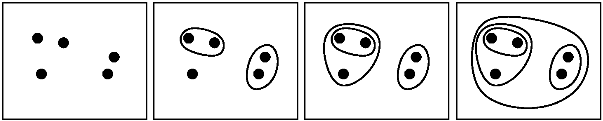
\includegraphics[width=0.7\linewidth]{figs/agglomerative.png}\\
    \end{center}
    \medskip

    We need a similarity measure between two clusters
    \begin{itemize}
        \item \textit{Ward}: Minimizes variance within merged clusters. Leads to equally sized clusters
        \item \textit{Average}: Minimizes average distances between their points
        \item \textit{Complete}: Minimizes maximun distance between their points
    \end{itemize}
\end{frame}

\begin{frame}{Other clustering algorithms}{Agglomerative clustering (II)}
    Agglomerative clustering is a special case of hierarchical clustering
    
    \bigskip

	\centering Dendrogram\\ 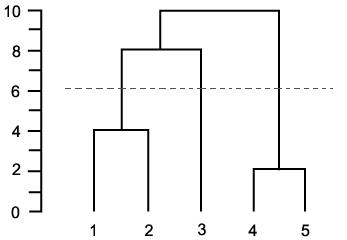
\includegraphics[width=0.5\linewidth]{figs/dendrogram.png}

	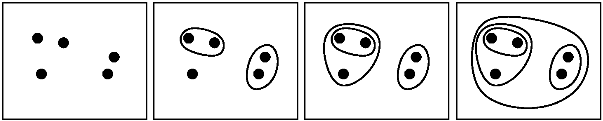
\includegraphics[width=0.7\linewidth]{figs/agglomerative.png}\\
	\scriptsize\href{https://stackoverflow.com/questions/8016313/agglomerative-clustering-in-matlab}{(Source)}
\end{frame}

\IfStrEq{\modo}{muii}{
    \subsection{Agglomerative clustering: Scikit-Learn}
    \begin{frame}{Other clustering algorithms}{Agglomerative clustering: Scikit-Learn}
        TODO: SCikit-Learn
    \end{frame}
}{}

\subsection{Agglomerative clustering: Summary}
\begin{frame}{Other clustering algorithms}{Agglomerative clustering: Summary}
	\begin{center}
	\begin{tabular}{cp{3cm}p{3cm}}\hline
	 	\texttt{Hyperparameters}  & \texttt{Advantages}  & \texttt{Disadvantages} \\\hline
	 	                 & Complex shapes                &  \\
	                     & Hierarchical clustering        &  \\
	 	                 &         &  \\
	 	\hline
	\end{tabular}
	\end{center}
\end{frame}

\section{Anomaly detection}

\begin{frame}{Anomaly detection}
    Two related concepts
    \begin{itemize}
        \item Outlayer detection and novelty detection
    \end{itemize}

    Adaptation of clustering and classification algorithms
    \begin{itemize}
        \item PCA, GMM, autoencoders, etc
    \end{itemize}

	\begin{center}
	\begin{tabular}{ccc}
	 	One-Class SVM & LOF    & Isolation Forest \\
	    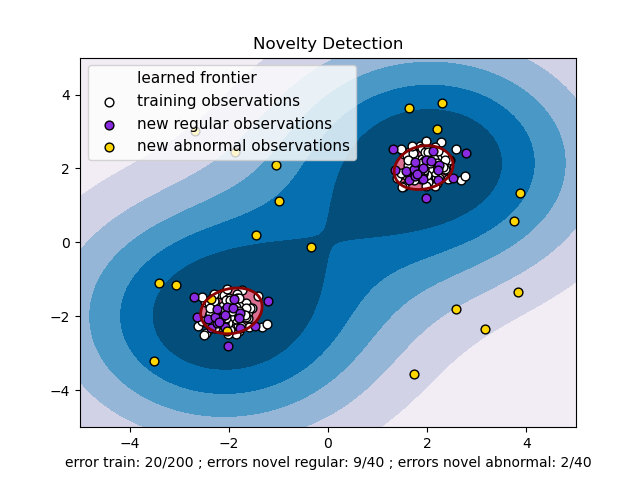
\includegraphics[width=0.33\textwidth]{figs/oneclasssvm.png} &
	    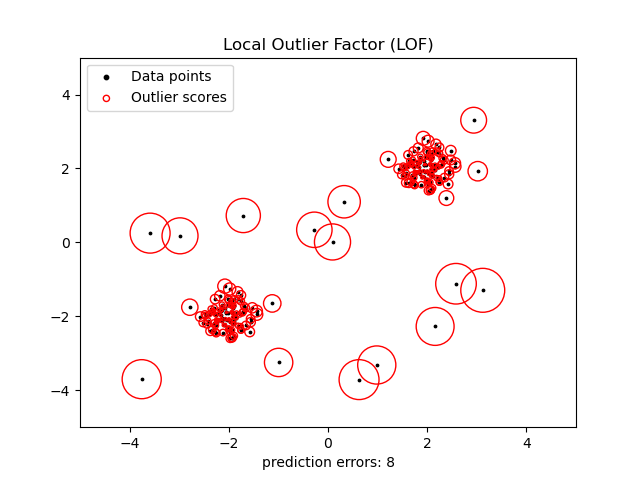
\includegraphics[width=0.33\textwidth]{figs/lof.png} &
	    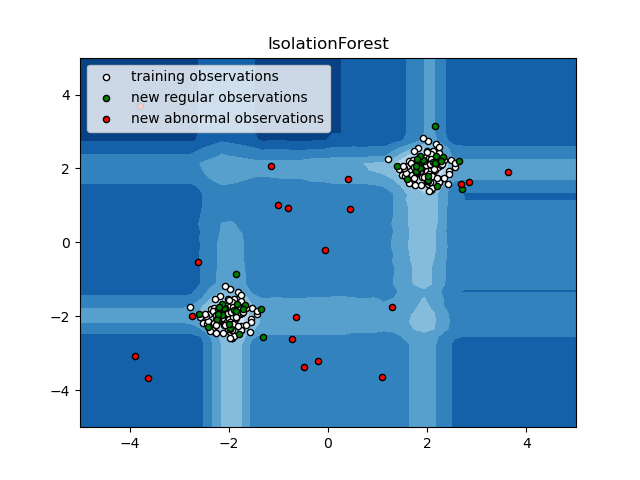
\includegraphics[width=0.33\textwidth]{figs/isolationforest.png} \\
	\end{tabular}
	\end{center}
	\centering \scriptsize\href{https://scikit-learn.org/stable/modules/outlier_detection.html}{(Source)}
\end{frame}


\section{Dimensionality reduction}
{
\sectionheaderWhite %Enclose the frame with {} and add this command for white background in section header
\begin{frame}{Dimensionality reduction}{PCA and manifold learning}
\end{frame}
}

\subsection{Main approaches for dimensionality reduction}

\begin{frame}{Dimensionality reduction}{Main approaches for dimensionality reduction (I)}
	Two main approaches to dimensionality reduction: Projection and \alert{manifold learning}

    \bigskip

    \centering Projection
    \begin{columns}
 	   \column{.5\textwidth}
	    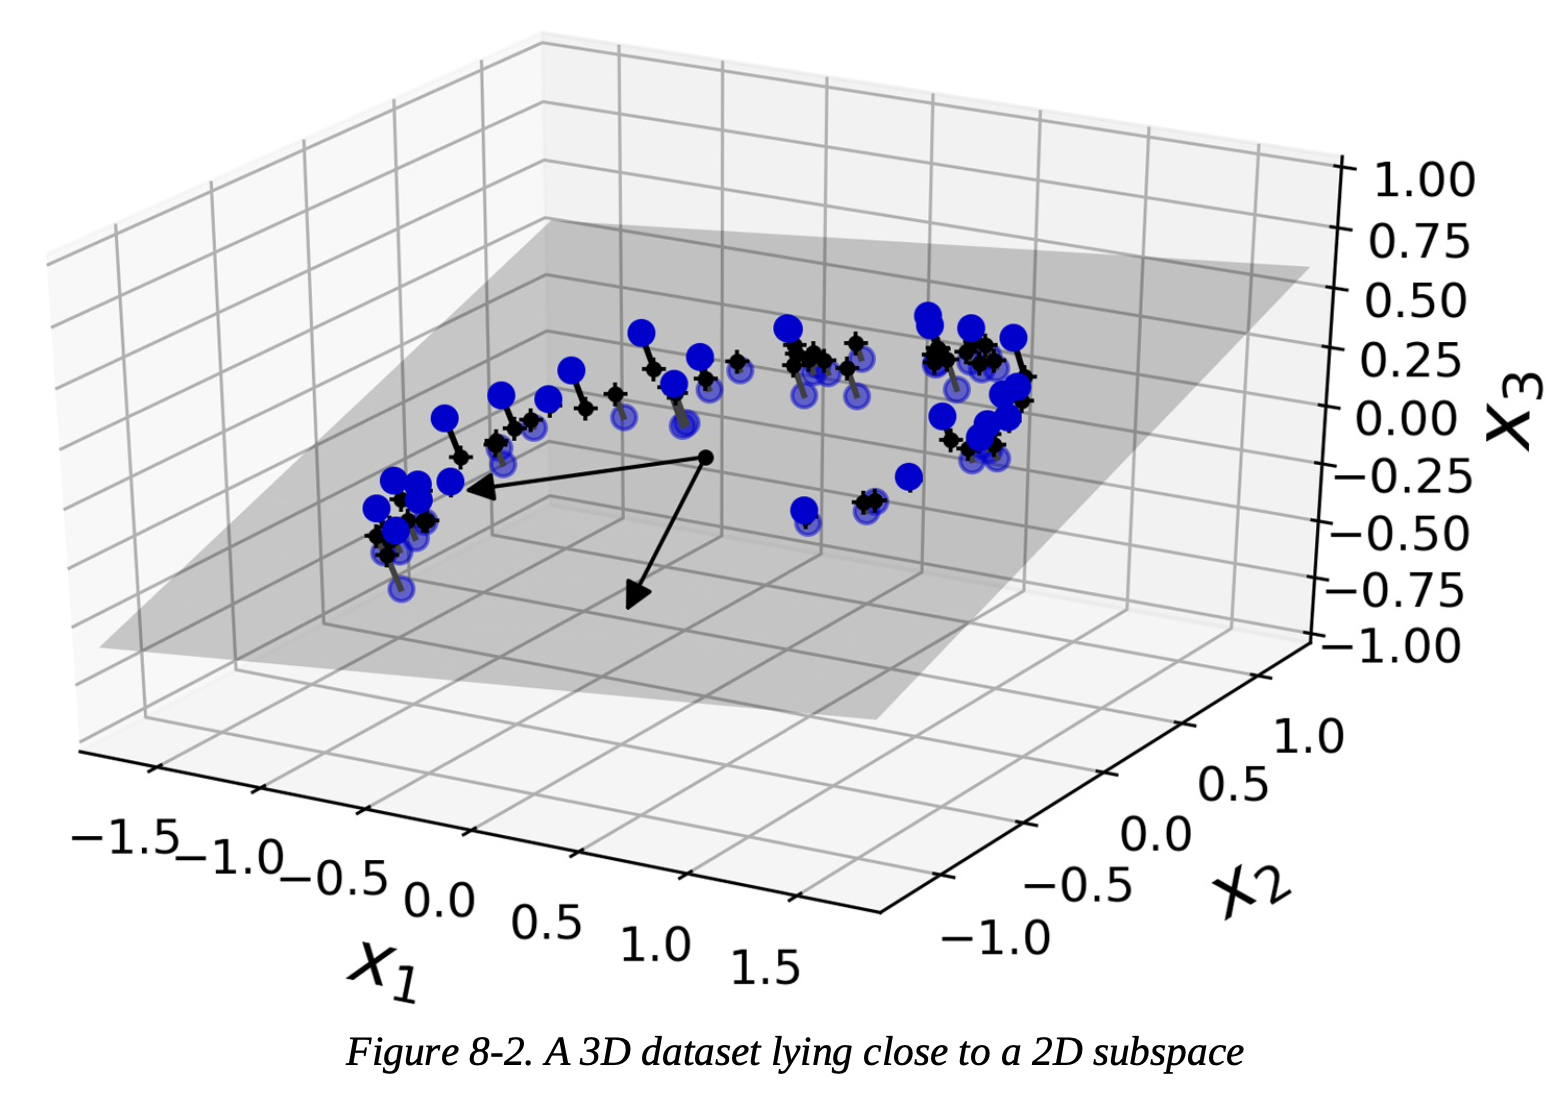
\includegraphics[width=\textwidth]{figs/subspace_projection.png} 
 	   \column{.5\textwidth}
	    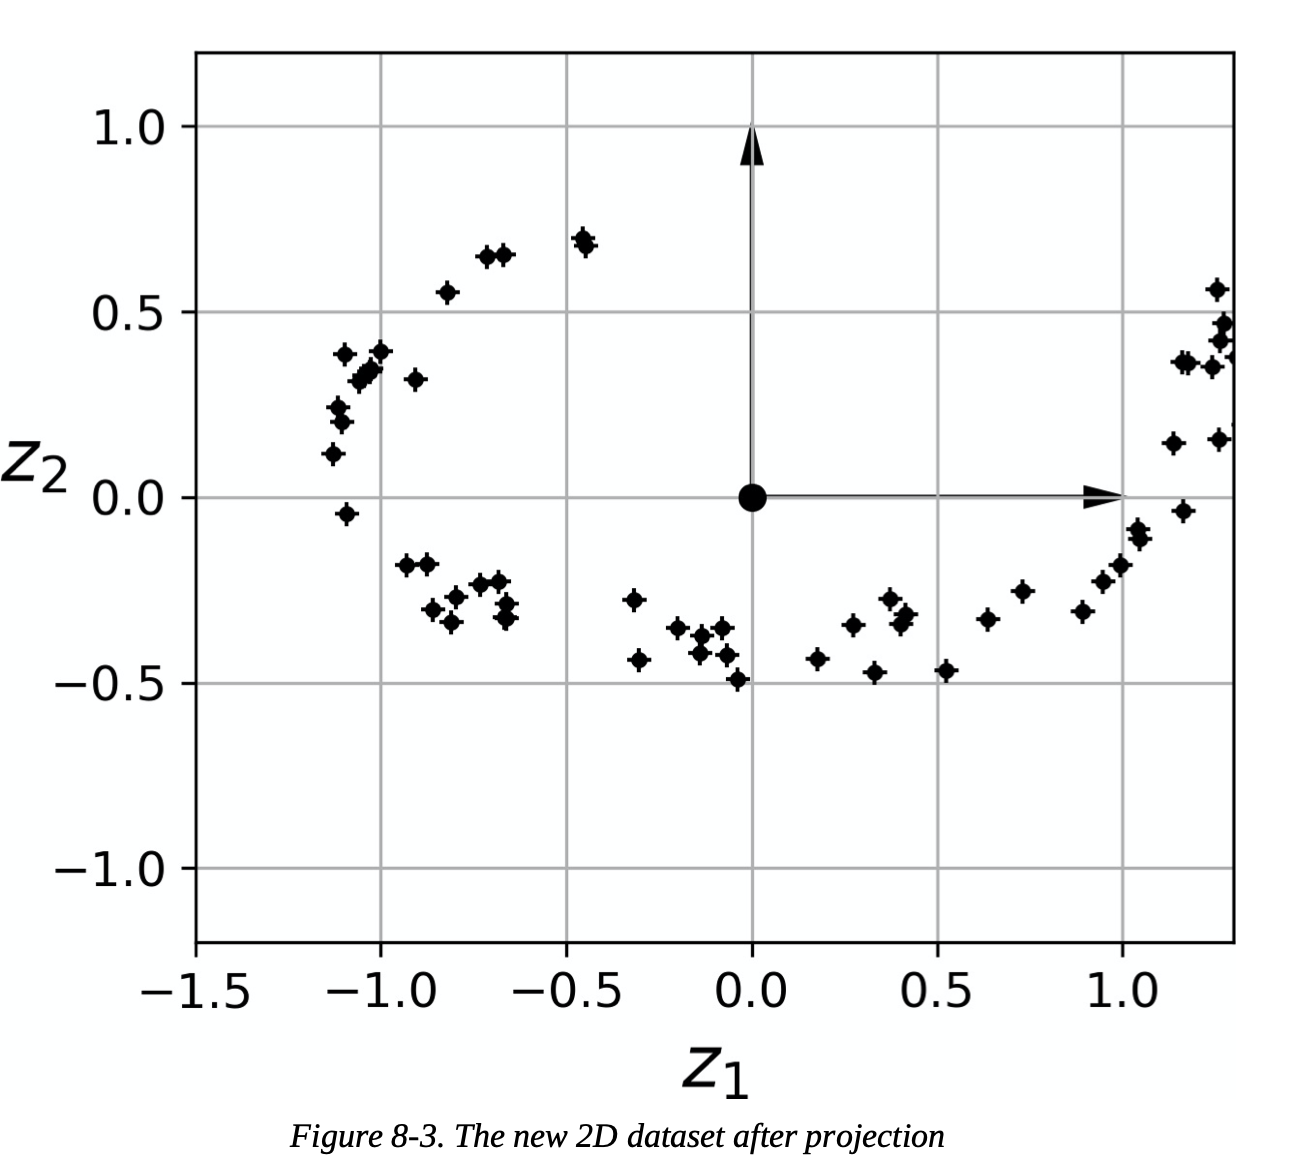
\includegraphics[width=\textwidth]{figs/2d_projection.png} 
    \end{columns}
	\scriptsize\href{https://github.com/Akramz/Hands-on-Machine-Learning-with-Scikit-Learn-Keras-and-TensorFlow/blob/master/08.Dim_Reduction.ipynb}{(Source)}

    \normalsize
    \flushleft
    Algorithms
	\begin{itemize}
		\item Principal Components Analysis (PCA), kernelized PCA, ...
	\end{itemize}
\end{frame}

\begin{frame}{Dimensionality reduction}{Main approaches for dimensionality reduction (II)}
    \centering Manyfold learning
    \begin{columns}
 	   \column{.5\textwidth}
	    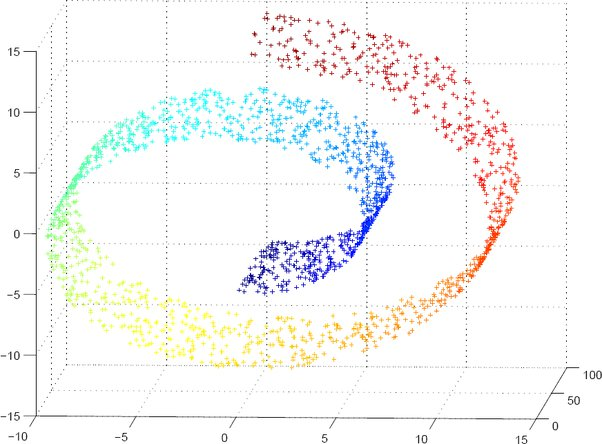
\includegraphics[width=\textwidth]{figs/manifold2.jpeg} 
 	   \column{.5\textwidth}
	    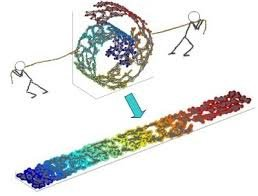
\includegraphics[width=\textwidth]{figs/manifold.jpeg} 
    \end{columns}
	\scriptsize\href{https://www.quora.com/What-is-manifold-learning}{(Source)}
    \normalsize
    \flushleft

    Manifold learning algorithms
    \begin{itemize}
		\item Isomap, T-distributed Stochastic Neighbor Embedding (t-SNE), Multi-dimensional Scaling (MDS), Locally Linear Embedding (LLE), ...
    \end{itemize}
\end{frame}



\begin{frame}{Dimensionality reduction}{Principal Components Analysis (I)}
	Dimensionality reduction transforms data into more convenient representations
	\begin{itemize}
		\item Reduce data dimensionality
		\item Visualize multidimensional data
	\end{itemize}

	Main algorithms

\end{frame}


\subsection{PCA}

\begin{frame}{Dimensionality reduction}{Principal Components Analysis (I)}
	Dimensionality reduction transforms data into more convenient representations
	\begin{itemize}
		\item Reduce data dimensionality
		\item Visualize multidimensional data
	\end{itemize}

	Main algorithms
	\begin{itemize}
		\item Isomap
		\item T-distributed Stochastic Neighbor Embedding (t-SNE)
		\item Principal Components Analysis (PCA)
	\end{itemize}

\end{frame}

\begin{frame}{Dimensionality reduction}{Principal Components Analysis (II)}
	PCA maximizes data variance

    \begin{columns}
 	   \column{.50\textwidth}
			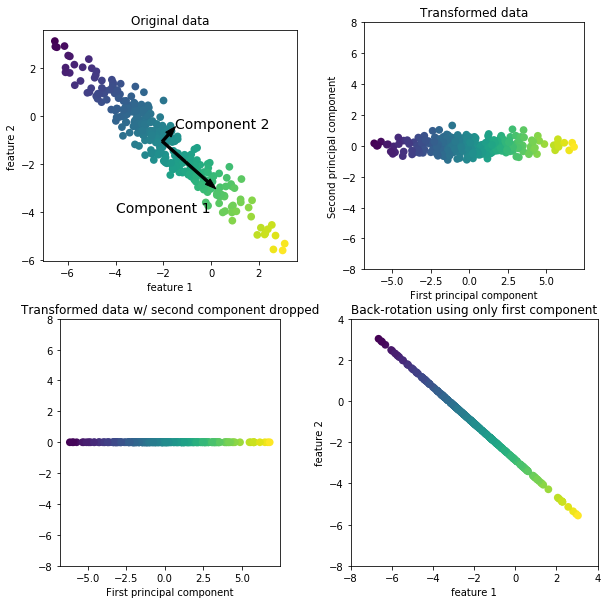
\includegraphics[width=\linewidth]{figs/pca.png}
    		\centering \tiny{\href{https://github.com/amueller/introduction_to_ml_with_python/blob/master/03-unsupervised-learning.ipynb}{(Source)}}
    \end{columns}
\end{frame}

\begin{frame}{Dimensionality reduction}{Principal Components Analysis (III)}
	\vspace{-0.5cm}
    \begin{columns}
 	   \column{.70\textwidth}
		Example: Hand-written digits recognition
		\begin{itemize}
			\item Images of hand-written digits
			\item 8x8 images (64 dimensions)
			\item $10$ digits
			\item Classification problem
		\end{itemize}
 	   \column{.30\textwidth}
			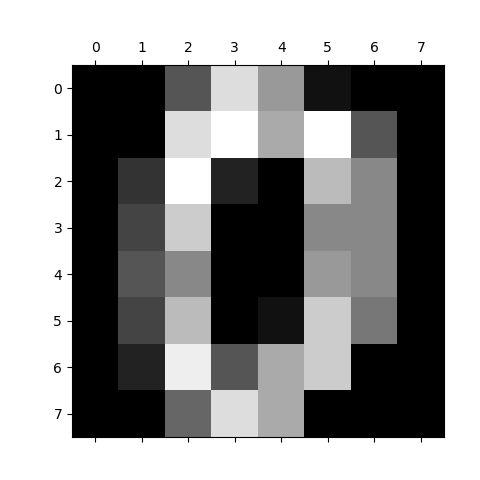
\includegraphics[width=\linewidth]{figs/zero.png}
    \end{columns}

    \begin{columns}
 	   \column{.50\textwidth}
			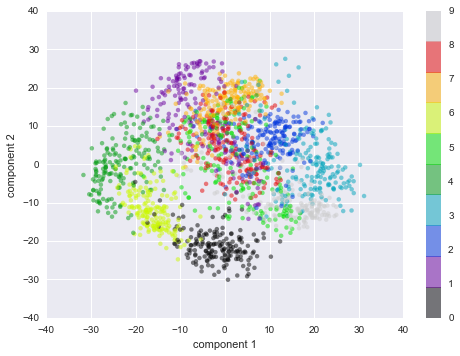
\includegraphics[width=\linewidth]{figs/handdigitspca.png}
 	   \column{.50\textwidth}
			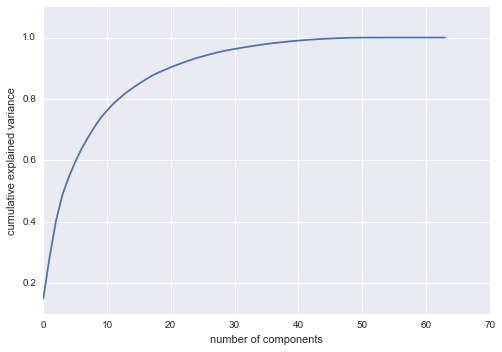
\includegraphics[width=\linewidth]{figs/pcacomponents.png}
    \end{columns}

   	\centering \tiny{\href{https://github.com/amueller/introduction_to_ml_with_python/blob/master/03-unsupervised-learning.ipynb}{(Source)}}
\end{frame}



\end{document}
